\section{延迟坐标}
\label{sec:2.6}
要考察正在奔驰之中的马群,最好是跳上一匹马背一起奔跑。类似地,要考察运动之
中的波,比较好的办法是沿着这些波一起移动。所以,为描述正在向下移动进入地层中去的
波,我们可以放弃$(x,z)$坐标而采用运动坐标$(x,z')$,其中$z'=z+tv$。

替代运动坐标系统的一种办法是定义延迟里标$(x,z,t')$,其中,$t'=t-z/v$。延迟
坐标的经典例子就是太阳时,飞机以太阳的速度向西飞行,则在飞机上看来,时间似乎是静
止不动的。

无论在运动坐标参照系还是在延迟坚标参照系内,偏移过程都与模拟波动传播过程类
似。铲迟坐标比运动坐标更为通用。理由就是:在固体地球物理学中,速度可能既与$x$有关
又与$z$有关,可是我们进行地震观测期间,地层却不随时间$t$而变;而在一个运动坐标系统
内,速度却可以与所有三个变量都有关,以致不必要地增加了计算的复杂性。Fourier变换
是求波动方程的一种通用工具,可是当系数不是常数时,它就没有多大用武之地了。


\subsection{独立变量定义}
\label{sec:2.6.1}
如何具体定义延迟坐标是个方便不方便的间题。延迟作周经常是建立在以速度$\bar{v}(z)$笔
直向下运动之假想射线的基础上,这些坐标的定义即使在速度横向可变(例如,速度为$v(x,z)$))
的问题中,也是有用处的。纵使并不存在严格的笔直向下传播的射线。原则上,可以利用任
何坐标系统去描述任何环境,不过,当用来定义它的射线族越来越偏离实际射线时,延迟坐
标系统的有效性一般就降低了。

尽管手头有现成的简单情形,但为使定义更正式和精确一点,还是值得花时间的。用普
通直角坐标$(t,x,z)$表示延迟坐标系$(t',x',z')$可按下列方程组来定义
\begin{subequations}
\begin{equation}
t'=t'(t,x,z)=t-\int_0^z\frac{dz}{\bar{v}(z)}
\label{eq:ex2.6.1a}
\end{equation}
\begin{equation}
x'=x'(t,x,z)=x
\label{eq:ex2.6.1b}
\end{equation}
\begin{equation}
z'=z'(t,x,z)=z
\label{eq:ex2.6.1c}
\end{equation}
\label{eq:ex2.6.1}
\end{subequations}
取积分的目的是将从地面至深度$z$的传播旅行时间累加起来;将$(x',z')$定义成刚好等于
$(x,z)$的原因,首先是为了进行偏微分时能避免混乱,其次是为以后的工作做好准备,在
下一步的工作中,射线族是更为一般化的情形。

\subsection{从属变量定义}
\label{sec:2.6.2}
有两类从属变量,即描述介质特征的那些变量和描述波特征的那些变量。介质特征用它
的速度和它的反射率$c$表示,波的特征则是利用上行波$U$、下行波$D$、压力$P$和压力的调制
形式$Q$表示。我们说,$P(t,x,z)$是给定$(t,x,z)$时的待求压力之数学函数形式, $P'(t',x',z')$
则是給定$(t',x',z')$时的数学函数形式。应这样表述这两个数学函数
$P$与$P'$全都属于相同物理变量
\begin{equation}
\begin{split}
P(t,x,z) &= P'[t'(t,x,z),x'(t,x,z),z'(t,x,z)]\\
P(t,x,z) &= P'(t',x',z')
\end{split}
\label{eq:ex2.6.2}
\end{equation}
显然,对于其他从属变量和像速度$v(x,z)$这样的介质参量,也存在类似的表达式。

\subsection{连锁法与高频板限}
\label{sec:2.6.3}

在$(t,x,z)$空间内,我们遇到的是熟悉的数学物理偏微分方程。偏微分连锁法(ch­ain rule)
将把偏导数转换至$(t',x',z')$空间。例如,对$z$来微分\ref{eq:ex2.6.2}, 得
\begin{subequations}
\begin{equation}
\frac{\partial P}{\partial z}=\frac{\partial P'}{\partial t'}\frac{\partial t'}{\partial z}+
\frac{\partial P'}{\partial x'}\frac{\partial x'}{\partial z}+
\frac{\partial P'}{\partial z'}\frac{\partial z'}{\partial z}
\label{eq:ex2.6.3a}
\end{equation}
利用式\ref{eq:ex2.6.1}计算出坐标导数,得
\begin{equation}
\frac{\partial P}{\partial z}=-\frac{1}{\bar{v}}\frac{\partial P'}{\partial t'}+
\frac{\partial P'}{\partial z'}
\label{eq:ex2.6.3b}
\end{equation}
\label{eq:ex2.6.3}
\end{subequations}
在式\ref{eq:ex2.6.3}中,关于变量$P$并没什么特别之处,我们也可写为
\begin{equation}
\frac{\partial }{\partial z}=-\frac{1}{\bar{v}}\frac{\partial }{\partial t'}+
\frac{\partial }{\partial z'}
\label{eq:ex2.6.4}
\end{equation}
式中,左端是对有关$(t,x,z)$的函数施行运算,而右端则是对与$(t',x',z')$有关之函数的运算。微分两次,得
\begin{equation}
\frac{\partial^2 }{\partial z^2}=(\frac{-1}{\bar{v}}\frac{\partial }{\partial t'}+\frac{\partial}{\partial z'})(\frac{-1}{\bar{v}}\frac{\partial}{\partial t'}+\frac{\partial}{\partial z'})
\label{eq:ex2.6.5}
\end{equation}
利用速度恒与时间无关的事实,得到下述结果
\begin{equation}
\frac{\partial^2 }{\partial z^2}=(\frac{1}{\bar{v}^2}\frac{\partial^2 }{\partial (t')^2}-(\frac{2}{\bar{v}}\frac{\partial^2}{\partial t'\partial z'}+\frac{\partial^2}{\partial (z')^2})+(\frac{1}{\bar{v}^2}\frac{d\bar{v}}{\partial z'})\frac{\partial}{\partial t'}
\label{eq:ex2.6.6}
\end{equation}
除了带有括号的最右端一项以外,可以说,将算子\ref{eq:ex2.6.4}
“平方”就得出了二阶导数。这最
后一项差不多总是在数据处理中被忽略不计,原因是它的影响类似于额外的具有实质性系数
梯度的一阶导数项的影响,正如\ref{sec:1.5}节所述,这样一些项形成要更仔细加以计算的振幅,如
果式\ref{eq:ex2.6.6}中最后一项不得不包括在内,则所有这类项看来就得从一开始就被包括在内。

\subsection{延迟坐标内的Fourier变换}
\label{sec:2.6.4}

已知一压力场$P(t,x,z)$时,我们可就它的任何独立变量或所有独立变量$(t,x,z)$
对它进行傅氏变换。同样,如在延迟坐标系内规定该压力场,我们可以对$(t',x',z')$进
行傅氏变换。既然$(t,x,z)$的傅氏对偶是$(\omega,k_x,k_z)$,则令$(t',x',z')$的对偶
为$(\omega',k_x',k_z')$看来是合适的;现在的问题是如何将$(\omega',k_x',k_z')$同熟悉的$(\omega,k_x,k_z)$
联系起来?在偏微分连锁法中包含了这个问题的答案,任何像\ref{eq:ex2.6.4}
这样的表达式,进行Fourier变换后就是
\begin{equation}
ik_z=-\frac{-i\omega'}{\bar{v}}+ik_z'
\label{eq:ex2.6.7}
\end{equation}
计算出所有其他导数,得到变换
\begin{subequations}
\begin{equation}
\omega = \omega '
\label{eq:ex2.6.8a}
\end{equation}
\begin{equation}
k_x=k_x'
\label{eq:ex2.6.8b}
\end{equation}
\begin{equation}
k_z=k_z'+\frac{\omega'}{\bar{v}}
\label{eq:ex2.6.8c}
\end{equation}
\label{eq:ex2.6.8}
\end{subequations}
记住,标量波动方程的波散关系为
\begin{equation}
\frac{\omega^2}{v^2}=k_x^2+k_z^2
\label{eq:ex2.6.9}
\end{equation}
将式\ref{eq:ex2.6.8}代入式\ref{eq:ex2.6.9},我们得到以延迟时间表示的标量波动方程表达式,即
\begin{equation}
(\frac{\omega'}{v})^2=(k_x')^2+(k_z'+\frac{\omega'}{\bar{v}})^2
\label{eq:ex2.6.10}
\end{equation}
在选取延迟作用速度等于介质速度的情形下,这两种波散关系如图\ref{fig:txz/rdisper}所示。
\begin{figure}[H]
\centering
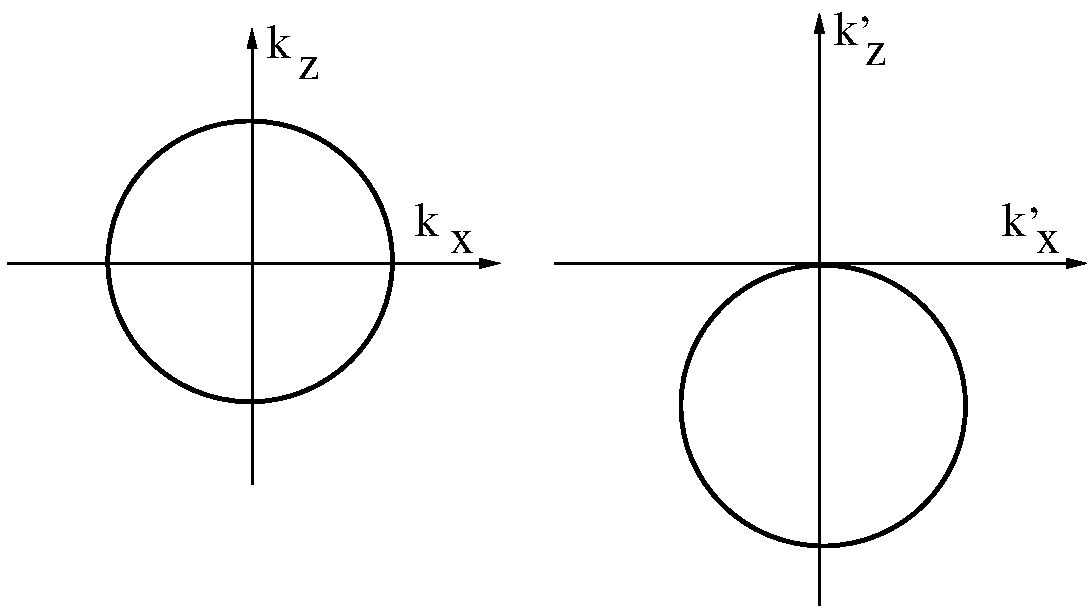
\includegraphics[width=0.65\textwidth]{txz/rdisper}
\caption[rdisper]{在通常坐标内(左图)和延迟时间坐标内(右图)的波动方程频散关系}
\label{fig:txz/rdisper}
\end{figure}
图\ref{fig:txz/rdisper}以图形方式阐明了延迟作用可以减少有限差分计算的时间。笔直向下
传播的波接近位于波散曲线(圆)顶部,
延迟的作用就是使圆的顶部向下移位至原
点。对$x$轴和$z$轴进行离散,将在这些轴上
引起空间频率假频;频率$\omega$越高,圆就越
大,移位后之圆的顶部显然就越易远离假频引起之折叠影响,另外,在$k_z'$超过
Nyquist频率$\pi/\Delta z$之前,可以使$\Delta z$增大(为节省计算时间起见)。

\subsection{对调制压力变量$\mathbf{Q}$的解释}
\label{sec:2.6.5}
